\chapter{User documentation}
\label{ch:user}

In this chapter we will discuss the installation steps,
the correct way of using the software and a brief description
about the software.


\section{Project Description}
\label{s:project_desc}

My project is a desktop application that is meant to run 
on the background while using Mastodon social media. The
whole project was built using the latest \textit{Python} 3 version.
The main goal of the project is to detect possible
threats coming from other accounts in form of direct
messages and tags, after warning the user about possible 
threats it let's the user decide the kind of action
he wants to take against the account that may be a threat
and the domain where the account came from.
\\[5pt]
This project is targeting all the ELTE server accounts, but with few modification
it will work for every server.
\\[5pt]
As a prerequisite for using this desktop application is
a stable internet connection and a Mastodon account.


\section{Installation guide}
\label{s:installation_guide}
As earlier mentioned, in order to use Mastodon social media threat alert application
we need to have a stable internet connection and a Mastodon account in any server and \textit{Python} 3.10.2.
\\[5pt]
The application is currently supporting Windows and Linux but the goal is to extend it as a 
mobile application which supports IOS and Android. Hence, the installation steps are the same for
both, Windows and Linux, but we will go through the steps in Windows specifically.
\\[5pt]
To download the application we need to clone the following repository: 
\url{https://github.com/DionKajdomcaj/Mastodon-Social-Threat-Alert.git}.
\\[5pt]
Prior to cloning the repository we need to make sure that we have git.
If git is missing, the user can download it at the
following url: \url{https://git-scm.com/download/win}.
If the git prerequisite is met, we can clone the repository by
running the following command in the command prompt:
\\[5pt]
\begin{lstlisting}[caption=Cloning Repository, captionpos=b]
	C:\Users\dionk>git clone https://github.com/DionKajdomcaj/Mastodon-Social-Threat-Alert.git
\end{lstlisting}
After succeeding to clone the repository we need to install the requirements for
our environment. In order to install the requirements we need to make sure we have
pip command. If the pip command is not installed, the user can install it by clicking
on the following url: \url{https://phoenixnap.com/kb/install-pip-windows}.
\\[5pt]
In the application folder there is a text file called requirements, installing it
will download all the libraries needed to run the application.
\\[5pt]
We can install them by using the following command in command prompt:
\\[5pt]
\begin{lstlisting}[caption=Installing requirements, captionpos=b]
	C:\Users\dionk\Mastodon-Social-Threat-Alert>pip install -r requirements.txt
\end{lstlisting}
Now we are ready to run the application, but prior to starting it,
it is highly recommended to clear the notifications the user has already
seen in Mastodon.
\subsection{Running the application}
\label{ss:running_app}
In order to run the application we need to make sure that
we are in the correct directory and then run the following command:
\\[5pt]
\begin{lstlisting}[caption=Running the application, captionpos=b]
	C:\Users\dionk\Mastodon-Social-Threat-Alert>python ThreatAlert.py 
\end{lstlisting}

After running the command, if all the prerequisites are met, we can see 
our application log in page, but the user must not close the command line while using the application since it will terminate the application.
\begin{figure}[H]
	\centering
	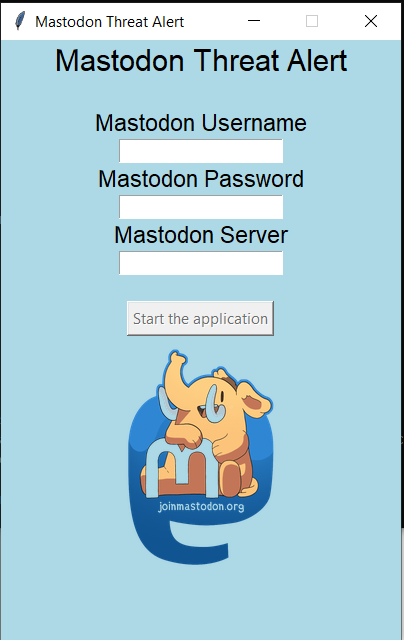
\includegraphics[width=0.3\textwidth,height=240px]{images/mainpageapp.png}
	\caption{Application main page}
	\label{fig:empty_page}
\end{figure}

\section{Logging in}
\label{s:Logging_in}
As we saw in figure \ref{fig:empty_page} the button to actually start the application is disabled.
In order to enable it we must fill all the necessary text fields which are:
\begin{itemize}
	\item \textbf{Mastodon username}, which is your original Mastodon account username.
	\item \textbf{Mastodon password}, which is your original Mastodon account password, that you use to log in to Mastodon.
	\item \textbf{Mastodon server}, which is the server your account is currently registered in.
\end{itemize}

If only one of the text fields is missing then the user will not be able
to start the application nor use it. 
\begin{figure}[H]
	\centering
	\subcaptionbox{Missing password field - Button disabled}{
		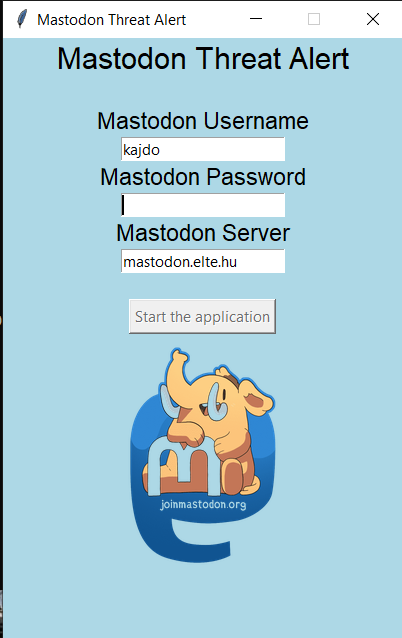
\includegraphics[width=0.3\textwidth, height=240px]{images/buttondisabled.png}}
	\hspace{5pt}
	\subcaptionbox{No missing field - Button enabled}{
		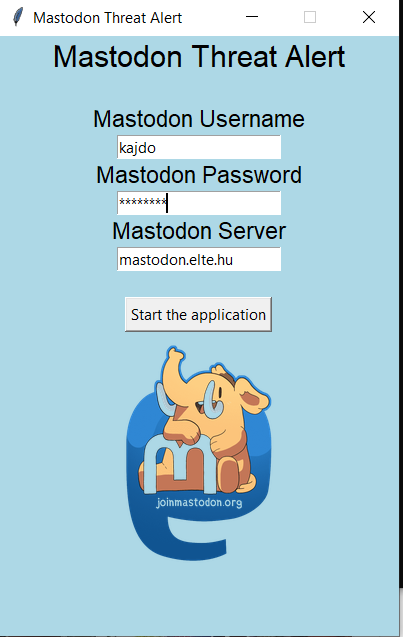
\includegraphics[width=0.3\textwidth, height=240px]{images/buttonenabled.png}}
	\caption{Button disabled and enabled}
	\label{fig:buttonenabled}
\end{figure}
The text fields must be filled with the Mastodon account information.
In the username field you must enter your Mastodon username, and the
same goes up to password. About the server you need to know which server
are you in and only type the domain, for example in case there is an account
like: \textbf{\url{example@mastodon.elte.hu}} then the username is \textbf{example} and the server is
\textbf{mastodon.elte.hu}. All of the data are case sensitive, so you must give them
exactly as they are originally.

\subsection{Valid log in data}
\label{ss:correct_data}
If every data is correct then the application will be connected to the Mastodon API after
we click on the button. But, prior to switching the screen it will show us a confirmation
message after API initialization. The API initialization takes a few seconds to be done so the user must wait during those seconds.
\begin{figure}[H]
	\centering
	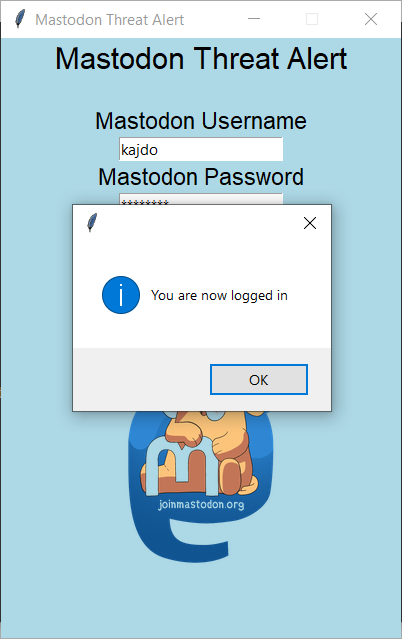
\includegraphics[width=0.3\textwidth,height=240px]{images/confimlogin.png}
	\caption{Confirmation window}
	\label{fig:confirm_logn}
\end{figure}
After closing the confirmation window, 
the program will let us know that it is running, and it will not
change it's state until it recognizes a possible threat for the logged in user.
\begin{figure}[H]
	\centering
	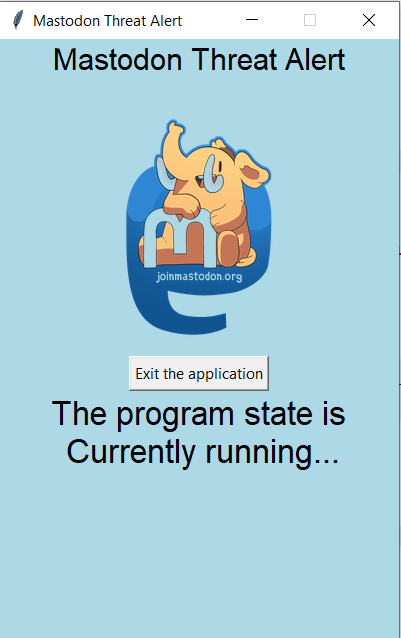
\includegraphics[width=0.3\textwidth,height=240px]{images/runningapp.png}
	\caption{Application running}
	\label{fig:running_app}
\end{figure}

\subsection{Invalid log in data}
\label{ss:incorrect_data}
Even if the button is enabled it does not mean that the log in data entered by the user
are correct. So, if the user does not give the valid log in data then the application 
will not be connected to Mastodon API. Hence, it will give the user an error message.
The following figure is going to show you the message you will receive for giving invalid 
log in data. After receiving the message you can just close the message window and try again
as many times as you need.
\begin{figure}[H]
	\centering
	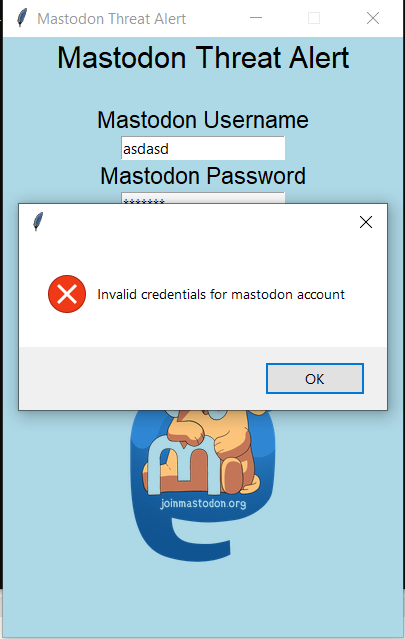
\includegraphics[width=0.3\textwidth,height=240px]{images/invalidred.png}
	\caption{Incorrect log in data}
	\label{fig:invalid_data}
\end{figure}
But if your account is not registered in "mastodon.elte.hu" domain then
even if your data is correct you will receive another error message.
\begin{figure}[H]
	\centering
	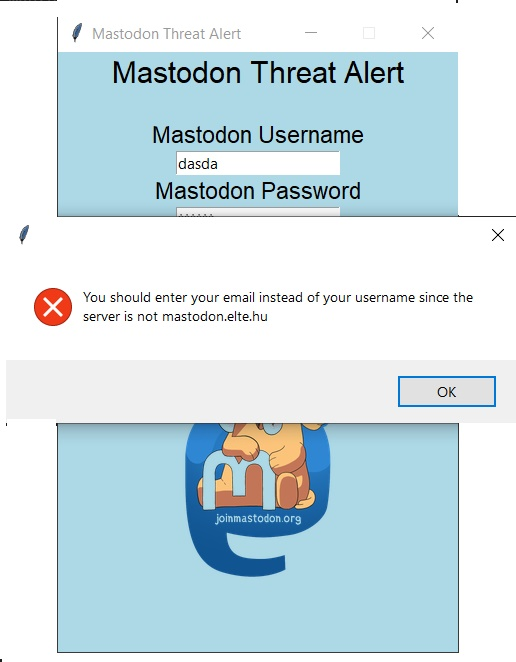
\includegraphics[width=0.4\textwidth,height=240px]{images/notelteserver3.jpg}
	\caption{User is not in ELTE server}
	\label{fig:not_elte}
\end{figure}
As we can see in \ref{fig:not_elte} if the server is not "mastodon.elte.hu" then
the email that your mastodon account is registered to should be given instead of
your username.

\section{Actions for the possible threat account}
\label{s:Actions_threat}
Now that we logged in successfully, we can start using Mastodon as usual, but this
time we have the Mastodon threat alert application running on the background and looking
for possible threats.
\\[5pt]
Every time that we are going to receive a direct message or a tag notification, that account's data is going to be checked whether it has a possibility to be a threat or not. After checking
if the account, that was trying to reach you, is considered to be a possible threat, the application
will show you a warning message containing the possible threat account's username and domain,
and will ask you to take a certain action against the account and the account's domain.
\begin{figure}[H]
	\centering
	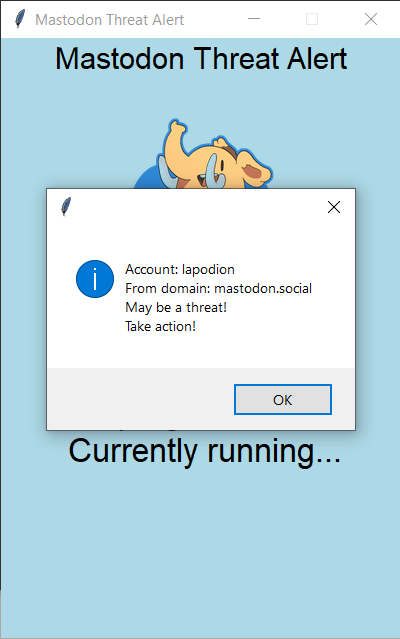
\includegraphics[width=0.3\textwidth,height=240px]{images/threatnotif.png}
	\caption{Possible threat notification}
	\label{fig:possible_threat_notification}
\end{figure}

We have three kind of actions supported in our application depending whether
we want to take them against an account or a domain. These actions are:
\begin{itemize}
	\item \textbf{Trust}
	\item \textbf{Block}
	\item \textbf{Mute}
\end{itemize}
The default value for both of them is Trust,  which can be changed.
\\[5pt]
We have to simply choose the action from a combo box for both, possible threat account and
it's domain, and click the button in order to perform the actions. 
\begin{figure}[H]
	\centering
	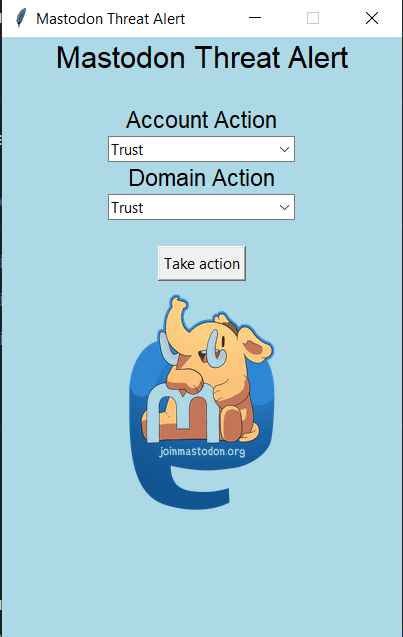
\includegraphics[width=0.3\textwidth,height=240px]{images/actionspage.png}
	\caption{Action window}
	\label{fig:action_page}
\end{figure}
Now we can choose independently the type of action for both, the account
and it's domain.
\\[5pt]
\begin{figure}[H]
	\centering
	\subcaptionbox{Account Actions}{
		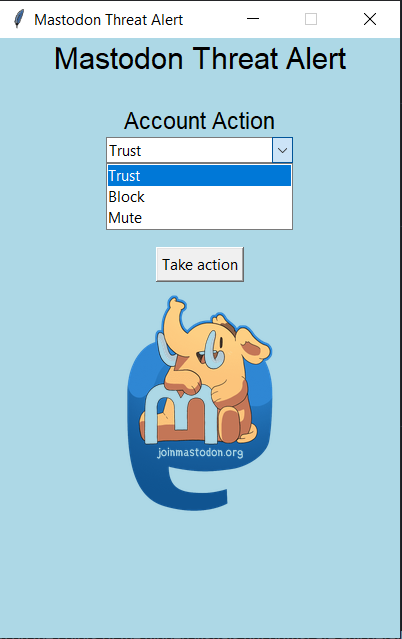
\includegraphics[width=0.3\textwidth, height=240px]{images/accountaction.png}}
	\hspace{5pt}
	\subcaptionbox{Domain Actions}{
		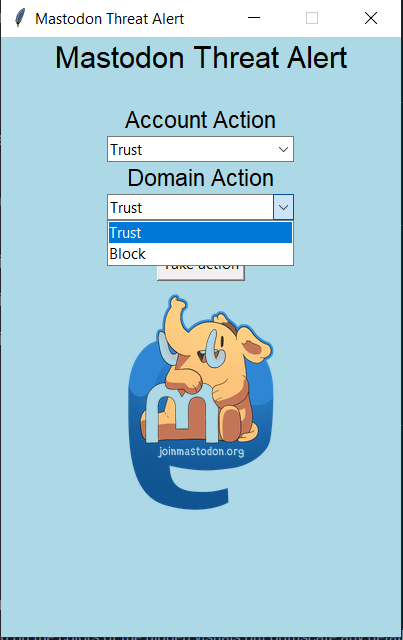
\includegraphics[width=0.3\textwidth, height=240px]{images/domainaction.png}}
	\caption{Actions available for account and domain}
	\label{fig:action_both}
\end{figure}
When we click the button, a pop up window will show up, letting
you know that the actions were successful.
\begin{figure}[H]
	\centering
	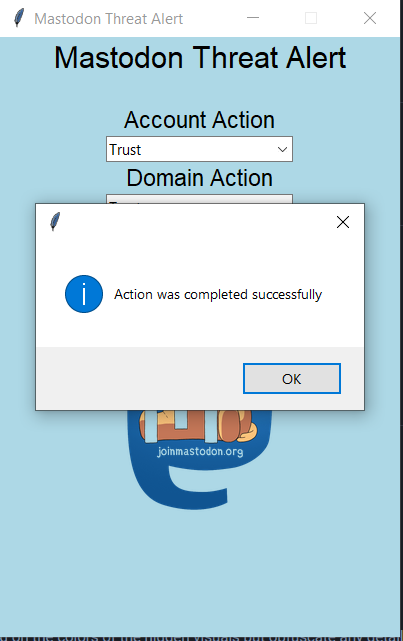
\includegraphics[width=0.3\textwidth,height=240px]{images/successaction.png}
	\caption{Pop up window to confirm the actions}
	\label{fig:pop_up_action}
\end{figure}
After closing the pop up window, the application will go back to
it's running state as in figure \ref{fig:running_app}.

\subsection{Account action}\label{ss:act_action}
As it was mentioned before, we can choose the actions separately for the possible threat account and it's
domain. In this section we are going to talk about the possible threat account's action.
\\[5pt]
We have 3 types of actions for the account, which are: Trust, Block, Mute.
The following table will describe each action.
\begin{center}
	\begin{longtable}{ | p{0.3\textwidth} | p{0.7\textwidth} | }
		
		\hline
		\multicolumn{2}{|c|}{\textbf{Account Actions}}
		\\ \hline
		

		\hline
		\endfirsthead % table header on first page
		
		\hline
		\hline
		\endhead % table header on further pages
		
		\hline
		\endfoot % table footer on previous pages
		
		\endlastfoot % table footer on last page
		
		\emph{Trust}
		& This action is very simple in context. When the user takes this action it means
		that he is trusting the possible threat account, and the application will not check the same account if it is trying to reach the user again.
		\\ \hline
		
		\emph{Block}
		& This action blocks the possible threat account, meaning it does not let the account reach the user anymore, not only by direct messaging or tagging, but even following, liking or any other social media activity. Besides those things the user will not see any activity from the possible threat account. To sum it up, the possible threat account will be non existent for the user.
		\\ \hline
		
		\emph{Mute}
		& Muting an account is same as ignoring the account, since the user will not receive notifications from the possible threat account anytime it tries to reach the user, but the user will still be able to check it's activity and the possible threat account will be able to try and reach the user, but simply the user will not be notified.
		\\ \hline
		
		\caption{Description of every action that can be taken against an account}
		\label{tab:account_ac_d}		
	\end{longtable}
\end{center}
However, every action that has been taken against the possible threat account can be easily reverted in Mastodon.
\subsection{Domain action}\label{ss:dmn_action}
In case of the possible threat account's domain we have less actions that can be taken against it. 
\\[5pt]
The actions are Trust and Block. They might seem the same as the account actions described in table \ref{tab:account_ac_d}, but blocking a domain is completely different, since here we are working with the whole domain. However, in case of Trust, the functionality is the same as it was in the possible threat account's action.
\\[5pt]
In the following table you can understand their functionality.
\begin{center}
	\begin{longtable}{ | p{0.3\textwidth} | p{0.7\textwidth} | }
		
		\hline
		\multicolumn{2}{|c|}{\textbf{Domain Actions}}
		\\ \hline
		
		
		\hline
		\endfirsthead % table header on first page
		
		\hline
		\hline
		\endhead % table header on further pages
		
		\hline
		\endfoot % table footer on previous pages
		
		\endlastfoot % table footer on last page
		
		\emph{Trust}
		& This action works the same way as it works to trust an account. However, trusting the domain will not take any actual action against the domain. So, simply the accounts that are from that domain can freely reach the user in any form and without any restrictions.
		\\ \hline
		
		\emph{Block}
		& In case of Block the whole activity of the domain accounts is blocked, meaning that the user won't see any of the accounts, that belong in that domain, activity. But, the user should always be very careful and is recommended not to block domains unless he/she was disturbed many times by the accounts coming from the same domain.
		\\ \hline

		\caption{Description of every action that can be taken against a domain}
		\label{tab:account_do_d}		
	\end{longtable}
\end{center}
Same as in the account actions, the domain actions can be reverted in Mastodon.
\section{Exiting the application}
As we can see in figure \ref{fig:running_app}, we can exit the application in two ways, by clicking the button named \textit{Exit the application} or by simply closing the window. It is recommended to exit the application by clicking the button because it is terminated safely, but sometimes when we want to exit it while we are not on the running page, we can exit the application by closing the window as well. However, it is not recommended to close the application while taking actions, like in figure \ref{fig:action_page}, because the possible threat account's will not be saved in the database and no action will be taken against the possible threat account and it's domain.




